\chapter{Arhitektura i dizajn sustava}

		\textit{ Arhitektura ima 3 podsustava:}
	\begin{itemize}
		\item 	\textit{Web preglednik}
		\item 	\textit{Web aplikacija na web poslužitelju}
		\item 	\textit{Baza podataka - PostgreSQL }		
	\end{itemize}


{\underline{Web preglednik} je ujedino i prevoditelj koda koji korisniku omogućuje pregledavanje sadržaja web aplikacije i interakciju s istim.}

{\underline{Web poslužitelj} prima HTTP (engl. Hyper
Text Transfer Protocol) zahtjeve od klijenta (preglednika) koji sadrže informacije o tome što klijent traži, kao što su primjerice URL, GET, POST... i vraća dohvaćeni resurs ako ga ima te vraća statusni kod koji daje informacije o uspješnosti zahtjeva.}

{Tehnologije korištene u našoj aplikaciji temelje se na Spring Bootu i Reactu. Aplikacija se sastoji od serverske komponente napisane u Javi (Spring Boot) i klijentske komponente napisane u JavaScriptu (React). Za razvojno okruženje koristimo IntelliJ, a baza koju koristimo za spremanje podataka o registriranim korisnicima i sve informacije o natjecanjima je PostgreSQL.}

{\underline{Web aplikacija} temelji se na arhitekturi Model-View-Controller (MVC). Ova arhitektura omogućuje organizaciju aplikacije u tri ključne komponente:}

\begin{itemize}
    \item \textbf{Model}: Ova komponenta predstavlja poslovnu logiku i podatke aplikacije. Model je implementiran u Java programskom jeziku (Spring Boot) i odgovoran je za upravljanje podacima, komunikaciju s bazom podataka te izračune i obrade podataka.
    
    \item \textbf{View}: Komponenta za prikaz podataka korisnicima. Prikazi se generiraju u Reactu, a omogućuju korisnicima interakciju s aplikacijom putem web preglednika. Prikazi se oblikuju pomoću HTML-a, CSS-a i JavaScripta.
    
    \item \textbf{Controller}: Kontroler je posrednik između Modela i Viewa. Ova komponenta upravlja korisničkim zahtjevima, prima ulazne podatke od korisnika te izvršava odgovarajuće akcije u Modelu. Kontroler također određuje koji prikaz treba biti poslan korisnicima.\\
\end{itemize}	

				
		\section{Baza podataka}
			

			
		{Koristimo relacijsku bazu podataka čije su gradivne jedinke tablice definirane imenom i skupom atributa za jednostavno upravljanje podacima. Baza podataka ove aplikacije sastoji se od sljedećih entiteta:}
	\begin{itemize}
		\item 	\textit{Korisnik}
		\item 	\textit{Natjecanje}
		\item 	\textit{Zadaci na natjecanju}
		\item 	\textit{Zadatak}				
	\end{itemize}
		
			\subsection{Opis tablica}
			

				{\textbf{Korisnik} - entitet sadržava sve važne informacije o korisniku: Korisničko ime, lozinku, ime, prezime, identifikator slike, email, tip korisnika (natjecatelj/voditelj), individualni sažetak, potvrda registracije, potvrda administratora. }
				
				
				\begin{longtblr}[
					label=none,
					entry=none
					]{
						width = \textwidth,
						colspec={|X[6,l]|X[6, l]|X[20, l]|}, 
						rowhead = 1,
					} %definicija širine tablice, širine stupaca, poravnanje i broja redaka naslova tablice
					\hline \SetCell[c=3]{c}{\textbf{Korisnik}}	 \\ \hline[3pt]
					 \SetCell{LightGreen}id & INT	&   jedinstveni identifikator korisnika	\\ \hline
					 \SetCell{LightBlue} username	& VARCHAR &   	izabrano korisničko ime\\ \hline 
					 \SetCell{LightBlue}email & VARCHAR &  e-mail adresa korisnika \\ \hline 
					 \SetCell{LightBlue}image-id & INT	&  	identifikator slike korisnika	\\ \hline
					 \SetCell{LightBlue}confirmation-hash & VARCHAR & individualni kod za registraciju \\ \hline
					 name & VARCHAR	&  	ime korisnika	\\ \hline 
					 lastname & VARCHAR	&  	prezime korisnika	\\ \hline 										
					 user-type & VARCHAR & natjecatelj ili voditelj natjecanja \\ \hline
					 password & VARCHAR	&  	šifra korisnika	\\ \hline 					 
					 confirmed & BOOLEAN & potvrđena registracija preko korisničkog emaila \\ \hline
					 confirmed-by-admin & BOOLEAN & potvrđena registracija preko administratorskog emaila \\ \hline
					   
\end{longtblr}


				{\textbf{Natjecanje} - entitet sadržava sve važne informacije o natjecanju: Id natjecanja, vrijeme početka, vrijeme završetka, broj zadataka, id voditelja natjecanja, identifikator pehara. U odnosu je Many-To-One s entitetom korisnik preko atributa voditelja natjecanja,. }
				
				
				\begin{longtblr}[
					label=none,
					entry=none
					]{
						width = \textwidth,
						colspec={|X[6,l]|X[6, l]|X[20, l]|}, 
						rowhead = 1,
					} %definicija širine tablice, širine stupaca, poravnanje i broja redaka naslova tablice
					\hline \SetCell[c=3]{c}{\textbf{Natjecanje}}	 \\ \hline[3pt]
					 \SetCell{LightGreen}id & INT	&   jedinstveni identifikator natjecanja	\\ \hline
					 \SetCell{LightBlue}image-id & INT	&  	identifikator slike pehara	\\ \hline
					  date-time-of-beginning	& TIMESTAMP &   vrijeme početka natjecanja	\\ \hline 
					 date-time-of-ending	& TIMESTAMP &   vrijeme završetka natjecanja	\\ \hline  
					 competition-maker-id & INT	&  	id voditelja natjecanja	\\ \hline 
	 				number-of-problems & INT	&  	broj zadataka u natjecanju	\\ \hline 
				\end{longtblr}

				{\textbf{Zadatak} - entitet sadržava sve važne informacije o zadatku. Sadrži atribute id, trajanje natjecanja, booleanski atribut is-private, broj bodova koje je moguće ostvariti, tip problema, tekst zadatka, naslov i id korisnika koji je napravio zadatak. S entitetom Korisnik je u odnosu Many-To-One preko atributa problem-maker-id.}
				
		\begin{longtblr}[
					label=none,
					entry=none
					]{
						width = \textwidth,
						colspec={|X[6,l]|X[6, l]|X[20, l]|}, 
						rowhead = 1,
					} %definicija širine tablice, širine stupaca, poravnanje i broja redaka naslova tablice
					\hline \SetCell[c=3]{c}{\textbf{Zadatak}}	 \\ \hline[3pt]
					 \SetCell{LightGreen} id & INT	&   jedinstveni identifikator zadatka	\\ \hline
				  \SetCell{LightBlue}problem-maker-id & INT	& identifikator vlasnika zadatka	\\ \hline 
					 duration &  NUMERIC	& trajanje zadatka	\\ \hline 
					 is-private &  BOOLEAN	& provjerava je li zadatak objavljen	\\ \hline 
					 problem-type &  INT	&  težina zadatka	\\ \hline 
					text &  VARCHAR	& tekst zadatka	\\ \hline 
					 title &  NUMERIC	& naslov zadatka	\\ \hline 
					 points & INT  & broj bodova zadatka \\ \hline

				\end{longtblr}

				{\textbf{Zadaci na natjecanju} - entitet sadržava sve važne informacije o odnosu zadatka i natjecanja na kojem se nalazi. Atributi: id natjecanja i id zadatka }

				
				\begin{longtblr}[
					label=none,
					entry=none
					]{
						width = \textwidth,
						colspec={|X[6,l]|X[6, l]|X[20, l]|}, 
						rowhead = 1,
					} %definicija širine tablice, širine stupaca, poravnanje i broja redaka naslova tablice
					\hline \SetCell[c=3]{c}{\textbf{Zadaci na natjecanju}}	 \\ \hline[3pt]
					 \SetCell{LightBlue}competition-id & INT	&    identifikator natjecanja (natjecanje.id)	\\ \hline
					 \SetCell{LightBlue} problem-id & INT	& identifikator zadatka	(problem.id) \\ \hline 
				\end{longtblr} 


				

				{\textbf{Primjeri za evaluaciju} - entitet sadržava id zadatka te vrijednost i ključ, odnosno na ovaj način se mapiraju rješenja zadataka. }

				
				\begin{longtblr}[
					label=none,
					entry=none
					]{
						width = \textwidth,
						colspec={|X[6,l]|X[6, l]|X[20, l]|}, 
						rowhead = 1,
					} %definicija širine tablice, širine stupaca, poravnanje i broja redaka naslova tablice
					\hline \SetCell[c=3]{c}{\textbf{Primjeri za evaluaciju}}	 \\ \hline[3pt]
					 \SetCell{LightGreen}problem-id & INT	&  jedinstveni identifikator zadatka	\\ \hline
					 vrijednost & VARCHAR	&  očekivani izlaz programa  \\ \hline 
					 ključ & VARCHAR	&  ulaz programa \\ \hline 
				\end{longtblr}
				
				{\textbf{Slike} - entitet sadržava id slike te bajt zapis slike. Na ovaj način spremamo slike korisnika i pehara }
				
				\begin{longtblr}[
					label=none,
					entry=none
					]{
						width = \textwidth,
						colspec={|X[6,l]|X[6, l]|X[20, l]|}, 
						rowhead = 1,
					} %definicija širine tablice, širine stupaca, poravnanje i broja redaka naslova tablice
					\hline \SetCell[c=3]{c}{\textbf{Slike}}	 \\ \hline[3pt]
					\SetCell{LightGreen} id & INT	&  jedinstveni identifikator slike	\\ \hline
					data & BYTEA &  binarni kod slike \\ \hline 

				\end{longtblr}
				
				
			
			\subsection{Dijagram baze podataka}
				
				\noindent {ER dijagram baze podataka prikazan na slici \ref{fig:erdijagram} sadrži vizualne slike ključeva: primarni ključ prikazan je ikonom ključa žute boje, strani ključ sivom bojom, a atributi označeni brojem 1 su alternativni ključevi. Prvi redak svake tablice entiteta predstavlja vidljivost tablice u bazi podataka, u drugom se retku nalazi ime tablice, a u preostalim retcima su ispisani atributi.
				}\\
					\begin{figure}[H]
					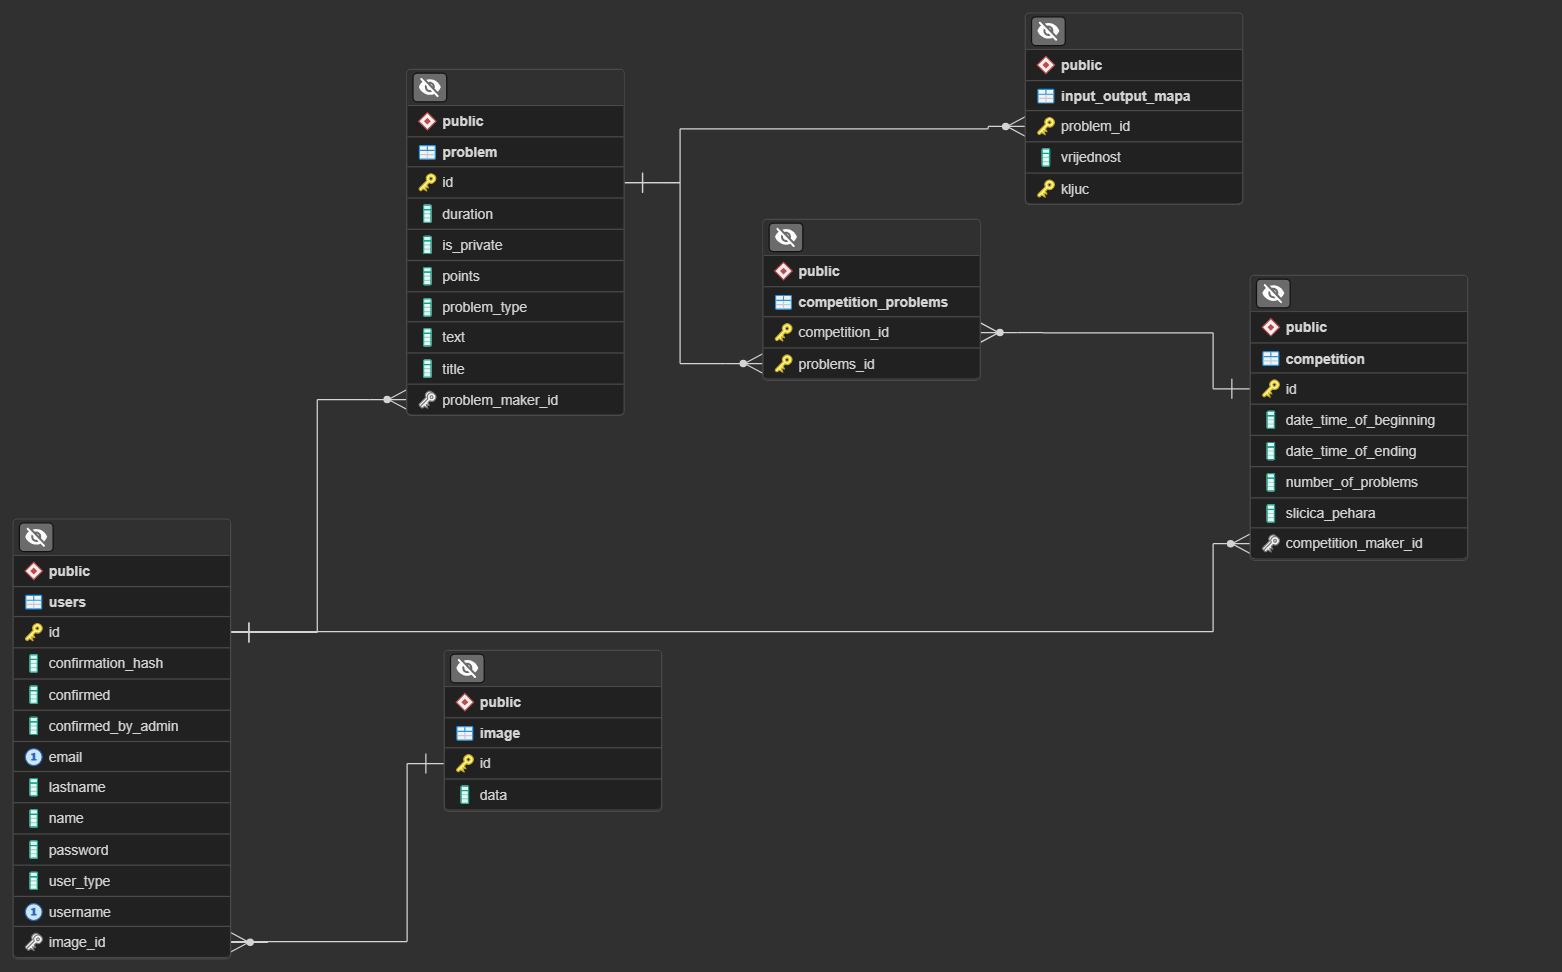
\includegraphics[scale=0.3]{slike/Er dijagram baze}
					%veličina slike u odnosu na originalnu datoteku i pozicija slike
					\centering
					\caption{Er dijagram baze podataka}
					\label{fig:erdijagram}
				\end{figure}
			
			\eject
			
			
		\section{Dijagram razreda}
		
			\noindent {U nastavku su prikazani razredi na kojima je zasnovan backend aplikacije.
				Lako je uočljivo da većina njih u nazivu sadrži naziv entiteta iz baze, te riječi Service i Controller. 
			}\\
				\begin{figure}[H]
				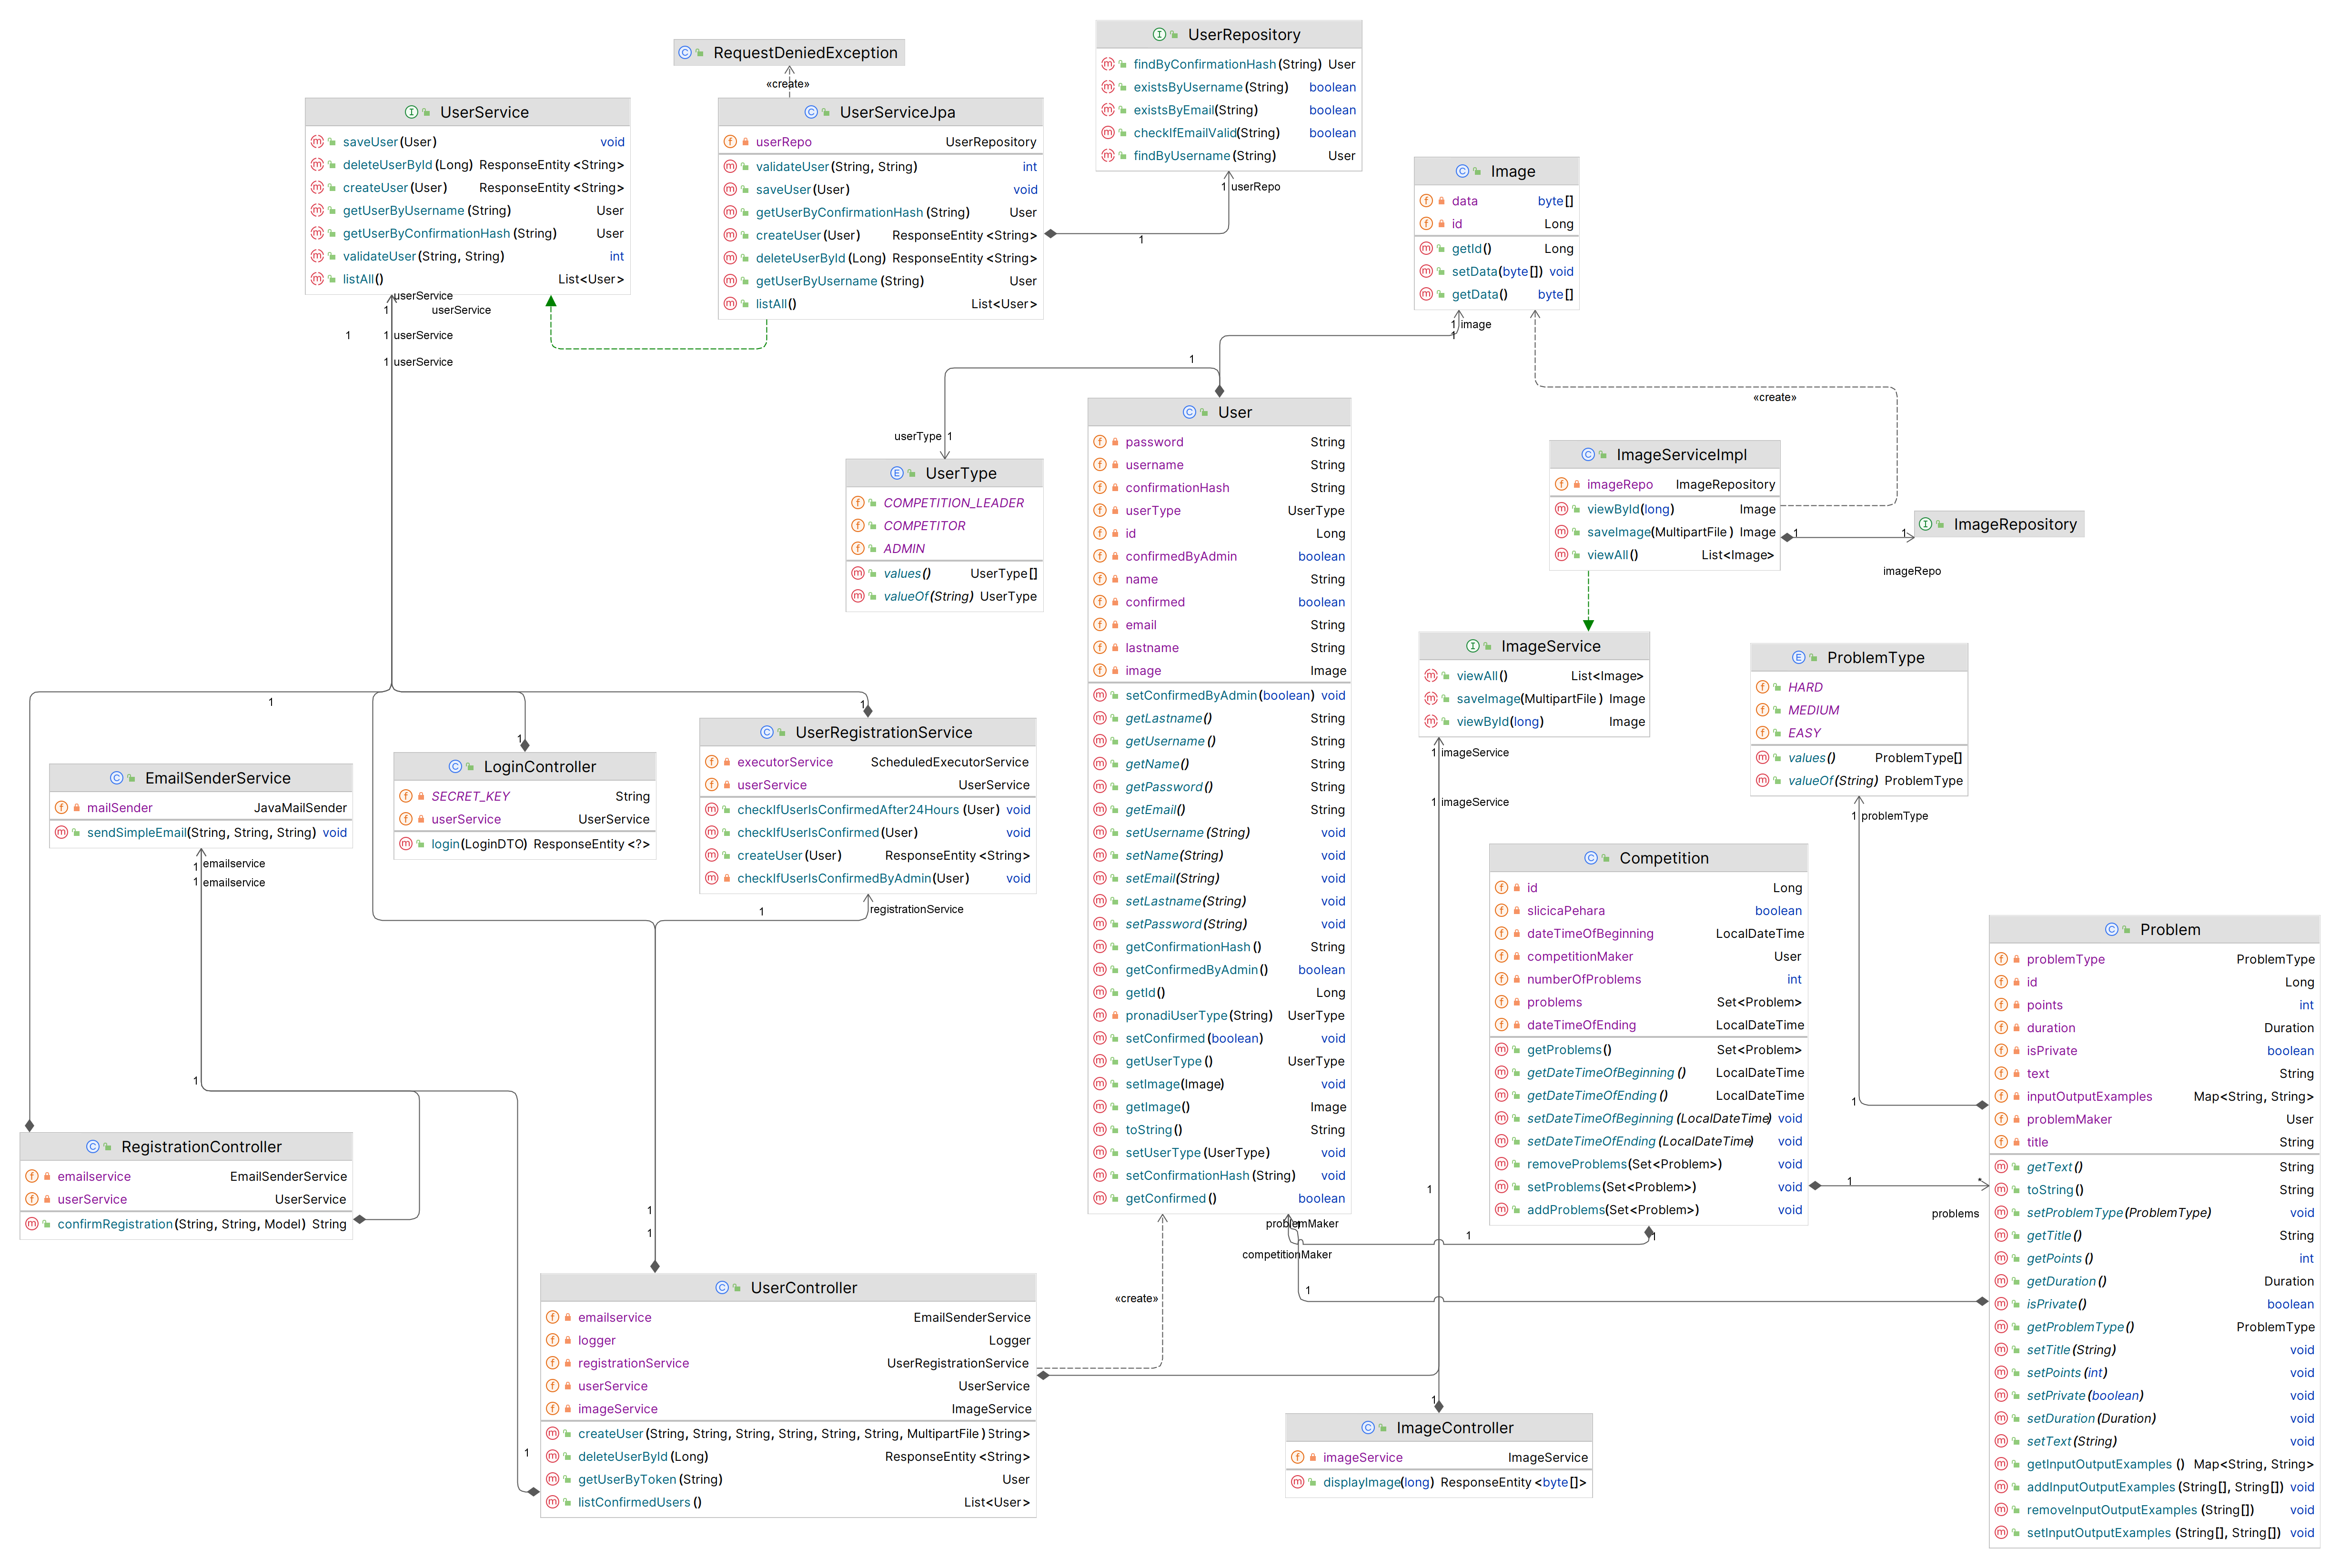
\includegraphics[scale=0.1]{slike/dijagramrazreda2}
				%veličina slike u odnosu na originalnu datoteku i pozicija slike
				\centering
				\caption{Dijagram razreda: razredi koji predstavljaju strukturu baze}
				\label{fig:dr2}
			\end{figure}
			
			\noindent{
				 Razredi User, Competition, Image i Problem sa slike \ref{fig:dr2} preslikavaju atribute svakog od entiteta iz baze. Razred User predstavlja registriranog korisnika, čiji UserType može biti COMPETITOR, COMPETITION LEADER i ADMIN (samo jedan, glavni korisnik), a koji pri registraciji unosi podatke prikazane na dijagramu (koji su vlastiti atributi razreda User). Razred Problem predstavlja zadatak koji je korisnik s tipom voditelj unio u sustav: na dijagramu se vidi ta poveznica. Jedna ili više instanci razreda Problem je dio Natjecanja tj. razreda Competition. Jedan korisnik može sudjelovati na više natjecanja, kao što i na jednom natjecanju sudjeluje jedan ili više korisnika. 
				Tu je i razred Image koji služi za pohranu slike u bazu podataka. 		
					
				Razredi imena Service služe za baratanje objektima razreda User, Competition itd. Razredi imena Controller obrađuju HTTP zahtjeve poslane na server i vraćaju zatražene podatke u .json obliku. 	
				
				 Strelice sa slike na jednostavan i intuitivan način prikazuju poveznice između razreda User, UserController i UserService. Metode koje su u razredima implementirane služe za baratanje entitetima u bazi: primarno su to razredi koji u svome nazivu sadrže 'Service' kao što je prije rečeno. Razred UserController oslanja se na ta dva prethodno navedena razreda da bi mogao ispuniti zaprimljene HTTP zahtjeve, bilo da je to samo informacija o korisnicima ili izmjena podataka.
				 
				 	Slika \ref{fig:dr1} prikazuje još neke Controller i Service razrede koji povezuju bazu i server. Prikazan je TokenService razred koji omogućava autentifikaciju korisnika, a time sadrži i informacije o njegovim ovlastima u aplikaciji. 
			}\\
			
			
			
		
			
			
			\begin{figure}[H]
				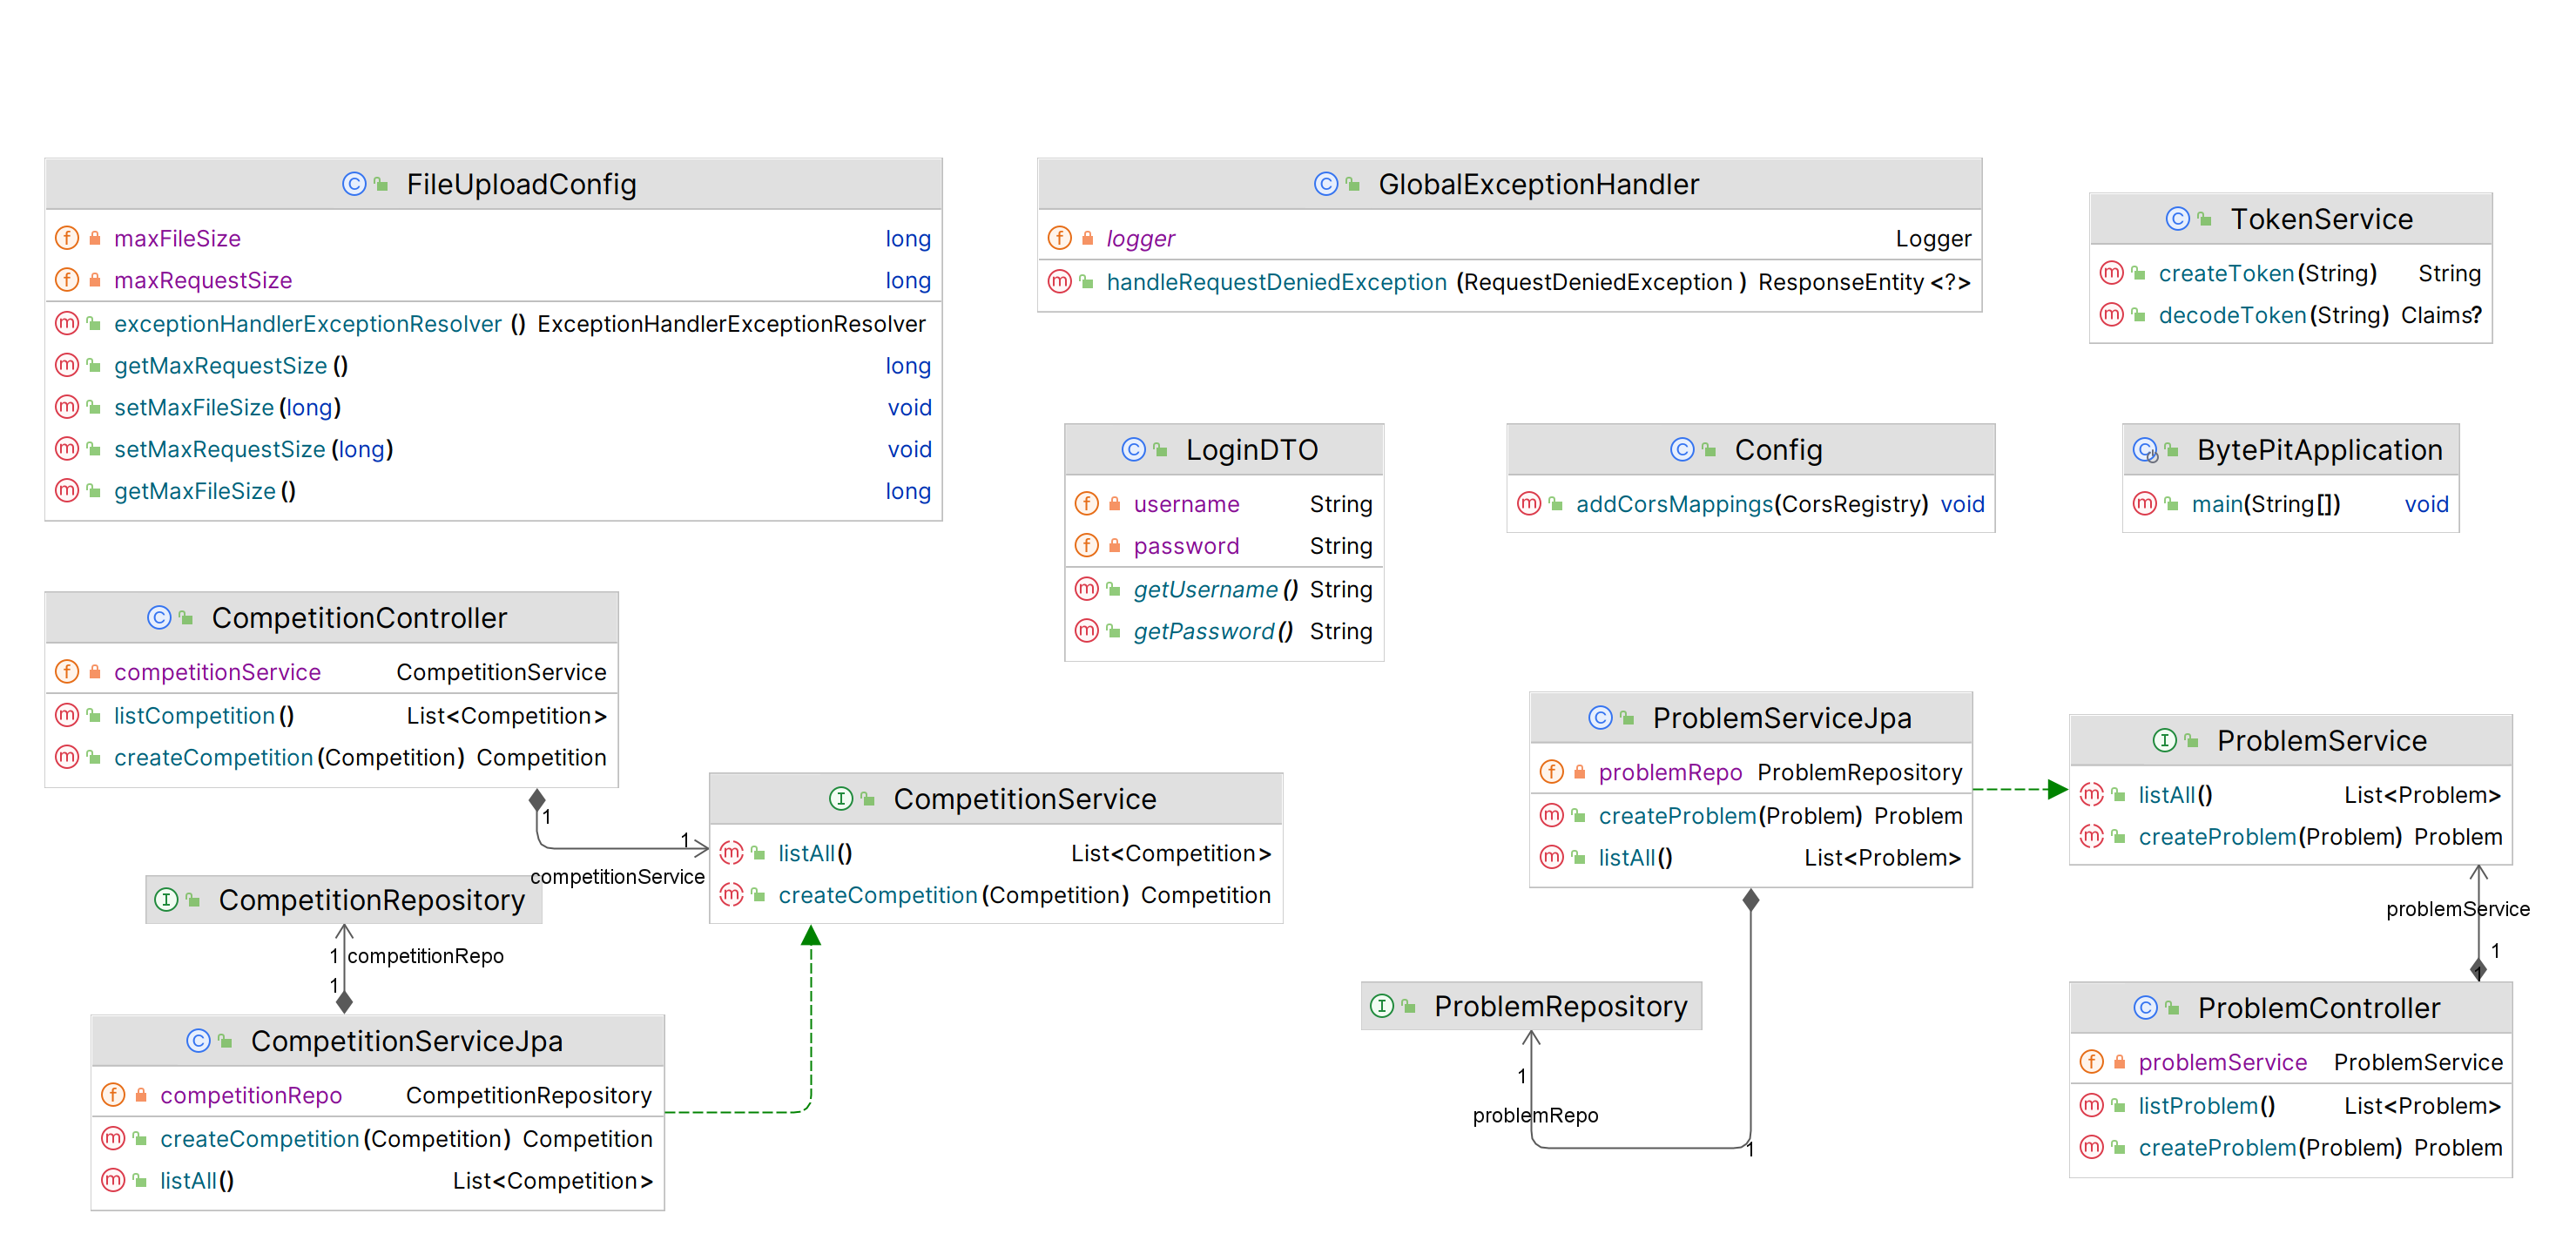
\includegraphics[scale=0.2]{slike/dijagramrazreda1}
				%veličina slike u odnosu na originalnu datoteku i pozicija slike
				\centering
				\caption{Dijagram razreda: ostali razredi Controller i Service te konfiguracija}
				\label{fig:dr1}
			\end{figure}
			
			
			
			\textbf{\textit{dio 2. revizije}}\\			
			
			\textit{Prilikom druge predaje projekta dijagram razreda i opisi moraju odgovarati stvarnom stanju implementacije}
			
			
			
			\eject
		
		\section{Dijagram stanja}
			
			
			\textbf{\textit{dio 2. revizije}}\\
			
			\textit{Potrebno je priložiti dijagram stanja i opisati ga. Dovoljan je jedan dijagram stanja koji prikazuje \textbf{značajan dio funkcionalnosti} sustava. Na primjer, stanja korisničkog sučelja i tijek korištenja neke ključne funkcionalnosti jesu značajan dio sustava, a registracija i prijava nisu. }
			
			
			\eject 
		
		\section{Dijagram aktivnosti}
			
			\textbf{\textit{dio 2. revizije}}\\
			
			 \textit{Potrebno je priložiti dijagram aktivnosti s pripadajućim opisom. Dijagram aktivnosti treba prikazivati značajan dio sustava.}
			
			\eject
		\section{Dijagram komponenti}
		
			\textbf{\textit{dio 2. revizije}}\\
		
			 \textit{Potrebno je priložiti dijagram komponenti s pripadajućim opisom. Dijagram komponenti treba prikazivati strukturu cijele aplikacije.}